\documentclass{beamer}
\mode<presentation>{
\usetheme{Warsaw}
\usecolortheme{sidebartab}
}
\usepackage{graphicx}
\usepackage{booktabs}
\title[Anonymity and encryption]{How to take back you privacy?}
\author{Naam, Genma}
\institute[@Gconfs]{
EPITA / Gconfs\\
\textit{naam@riseup.net\\ genma@riseup.net}
}
\date{01/17/13}
\usepackage[utf8]{inputenc}
\usepackage[T1]{fontenc}
\begin{document}
\begin{frame}
\titlepage
\end{frame}
\begin{frame}
\frametitle{Overview}
\tableofcontents
\end{frame}
\section{Intro}
\subsection{Why we do this talk?}
%---------------------------------------------------
\begin{frame}
\frametitle{Sensitive data}
\begin{block}{Definition}
\begin{itemize}
\item a set of values of qualitative or quantitative variables
\item individual pieces of information
\end{itemize}
\end{block}
Some of them are (important|critical)s, don't play with Mallory.
\end{frame}
%---------------------------------------------------
\begin{frame}
\frametitle{The right to stay anonymous}
The Convention for the Protection of Human Rights and Fundamental Freedoms states
that :
\begin{block}{Article 8 - Right to respect for private and family life}
\begin{itemize}
\item Everyone has the right to respect for his private and family life (...).
\item  There shall be no interference by a public authority with the exercise
of this right except such as is in accordance with the law and is necessary in
a democratic society \emph{in the interests of national security, public safety or
the economic well-being of the country, for the prevention of disorder or crime,
for the protection of health or morals, or for the protection of the rights and
freedoms of others}.
\end{itemize}
\end{block}
\end{frame}
%--------------------------------------------------
\begin{frame}
\frametitle{You will also see}
\begin{itemize}
\item Tons of softwares, distributions, techniques to defeat too inquisitive
people and censorship.
\item What's a Cryptoparty and what you could learn from it.
\end{itemize}
\end{frame}
%--------------------------------------------------

\subsection{The digital identity}
%--------------------------------------------------
\begin{frame}
\end{frame}
%--------------------------------------------------

\subsection{Questions?}
%--------------------------------------------------
\begin{frame}
\frametitle{Something unclear ?}
\begin{columns}[c]
\column{.5\textwidth}
\begin{figure}
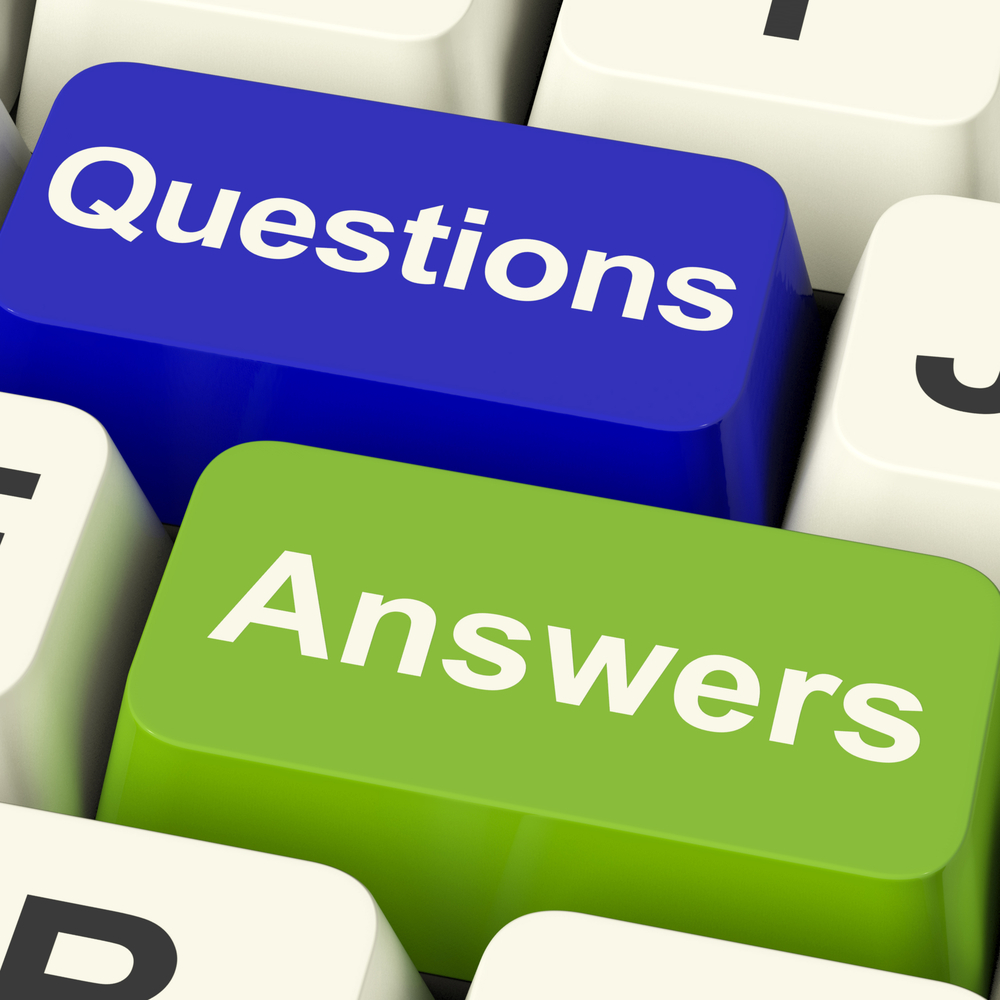
\includegraphics[width=0.8\linewidth]{./materials/questions}
\end{figure}
\column{.5\textwidth}
Feel free to ask for questions now.
\end{columns}
\end{frame}
%--------------------------------------------------

\section{HOW TO: Encryption}
\subsection{WTF is encryption?}
%--------------------------------------------------
\begin{frame}
\end{frame}
%--------------------------------------------------

\subsection{What can I encrypt? How?}
%--------------------------------------------------
\begin{frame}
\end{frame}
%--------------------------------------------------

\subsection{Questions?}
%--------------------------------------------------
\begin{frame}
\frametitle{Something unclear ?}
\begin{columns}[c]
\column{.5\textwidth}
\begin{figure}
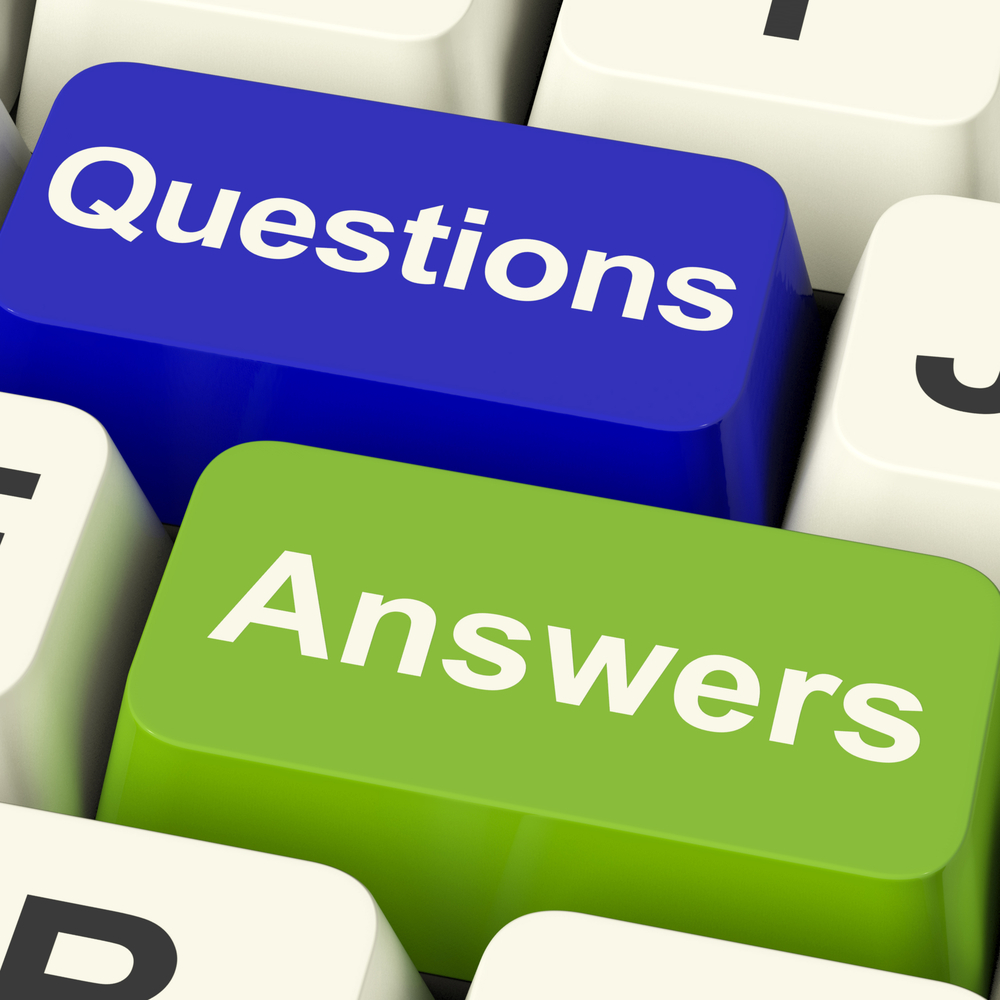
\includegraphics[width=0.8\linewidth]{./materials/questions}
\end{figure}
\column{.5\textwidth}
Feel free to ask for questions now.
\end{columns}
\end{frame}
%--------------------------------------------------

\section{HOW TO: Anonymity}
\subsection{Why does it matter?}
%--------------------------------------------------
\begin{frame}
\end{frame}
%--------------------------------------------------

\subsection{There is always a tool that fit your need}
%--------------------------------------------------
\begin{frame}
\end{frame}

\subsection{Questions?}
%--------------------------------------------------
\begin{frame}
\frametitle{Something unclear ?}
\begin{columns}[c]
\column{.5\textwidth}
\begin{figure}
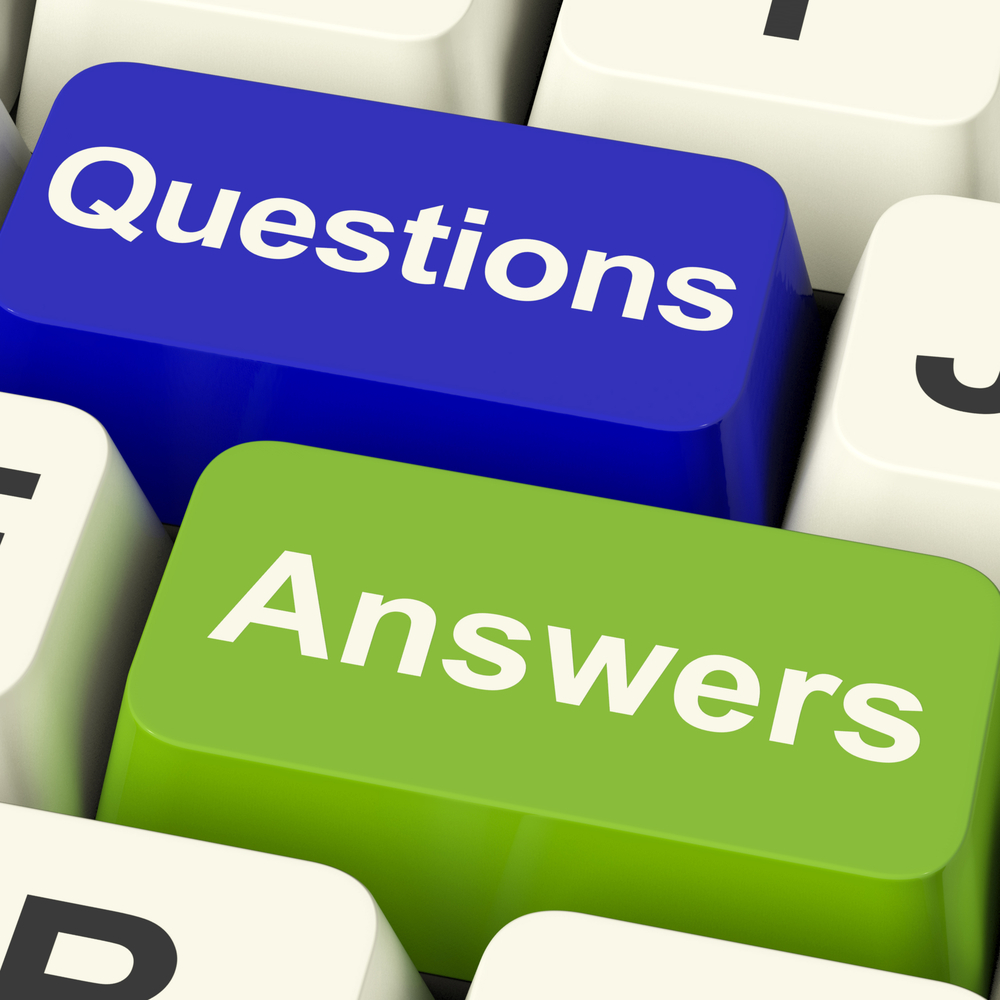
\includegraphics[width=0.8\linewidth]{./materials/questions}
\end{figure}
\column{.5\textwidth}
Feel free to ask for questions now.
\end{columns}
\end{frame}

%--------------------------------------------------
\section{Conclusion}
\subsection{We're not in a XOXO word}
%--------------------------------------------------
\begin{frame}
\end{frame}
%--------------------------------------------------

\subsection{Cryptoparty}
%--------------------------------------------------
\begin{frame}
\end{frame}
%--------------------------------------------------

\subsection{Questions?}
%--------------------------------------------------
\begin{frame}
\frametitle{Something unclear ?}
\begin{columns}[c]
\column{.5\textwidth}
\begin{figure}
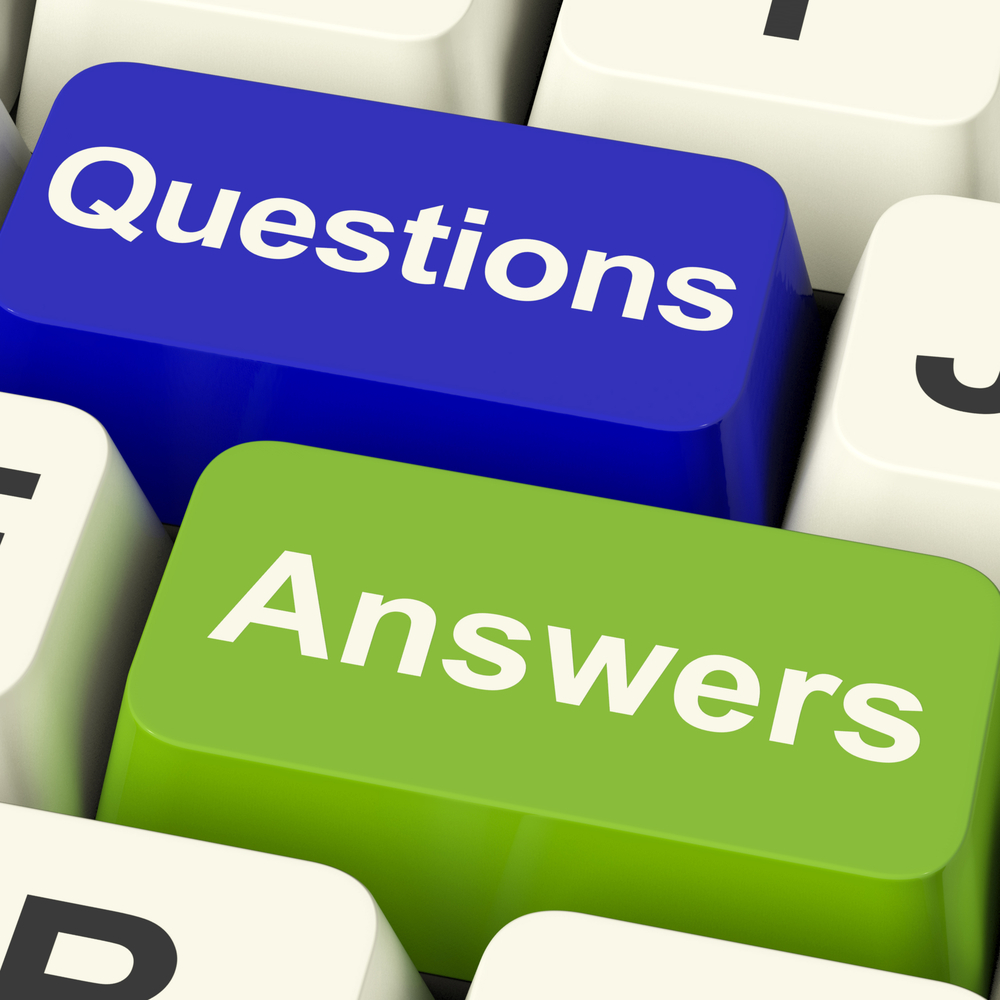
\includegraphics[width=0.8\linewidth]{./materials/questions}
\end{figure}
\column{.5\textwidth}
Feel free to ask for questions now.
\end{columns}
\end{frame}

%--------------------------------------------------
\begin{frame}
\frametitle{Rendez vous at the Cryptoparty}
\begin{figure}

\includegraphics[width=0.8\linewidth]{./materials/cryptoparty}
\end{figure}
\end{frame}
%--------------------------------------------------

\end{document}

